%% BioMed_Central_Tex_Template_v1.06
%%                                      %
%  bmc_article.tex            ver: 1.06 %
%                                       %

%%IMPORTANT: do not delete the first line of this template
%%It must be present to enable the BMC Submission system to
%%recognise this template!!

%%%%%%%%%%%%%%%%%%%%%%%%%%%%%%%%%%%%%%%%%
%%                                     %%
%%  LaTeX template for BioMed Central  %%
%%     journal article submissions     %%
%%                                     %%
%%          <8 June 2012>              %%
%%                                     %%
%%                                     %%
%%%%%%%%%%%%%%%%%%%%%%%%%%%%%%%%%%%%%%%%%


%%%%%%%%%%%%%%%%%%%%%%%%%%%%%%%%%%%%%%%%%%%%%%%%%%%%%%%%%%%%%%%%%%%%%
%%                                                                 %%
%% For instructions on how to fill out this Tex template           %%
%% document please refer to Readme.html and the instructions for   %%
%% authors page on the biomed central website                      %%
%% http://www.biomedcentral.com/info/authors/                      %%
%%                                                                 %%
%% Please do not use \input{...} to include other tex files.       %%
%% Submit your LaTeX manuscript as one .tex document.              %%
%%                                                                 %%
%% All additional figures and files should be attached             %%
%% separately and not embedded in the \TeX\ document itself.       %%
%%                                                                 %%
%% BioMed Central currently use the MikTex distribution of         %%
%% TeX for Windows) of TeX and LaTeX.  This is available from      %%
%% http://www.miktex.org                                           %%
%%                                                                 %%
%%%%%%%%%%%%%%%%%%%%%%%%%%%%%%%%%%%%%%%%%%%%%%%%%%%%%%%%%%%%%%%%%%%%%

%%% additional documentclass options:
%  [doublespacing]
%  [linenumbers]   - put the line numbers on margins

%%% loading packages, author definitions

\documentclass[twocolumn]{bmcart}% uncomment this for twocolumn layout and comment line below
%\documentclass{bmcart}

%%% Load packages
\usepackage{amsthm,amsmath}
%\RequirePackage{natbib}
%\RequirePackage[authoryear]{natbib}% uncomment this for author-year bibliography
\RequirePackage{hyperref}
\usepackage[utf8]{inputenc} %unicode support
%\usepackage[applemac]{inputenc} %applemac support if unicode package fails
%\usepackage[latin1]{inputenc} %UNIX support if unicode package fails


%%%%%%%%%%%%%%%%%%%%%%%%%%%%%%%%%%%%%%%%%%%%%%%%%
%%                                             %%
%%  If you wish to display your graphics for   %%
%%  your own use using includegraphic or       %%
%%  includegraphics, then comment out the      %%
%%  following two lines of code.               %%
%%  NB: These line *must* be included when     %%
%%  submitting to BMC.                         %%
%%  All figure files must be submitted as      %%
%%  separate graphics through the BMC          %%
%%  submission process, not included in the    %%
%%  submitted article.                         %%
%%                                             %%
%%%%%%%%%%%%%%%%%%%%%%%%%%%%%%%%%%%%%%%%%%%%%%%%%

\RequirePackage{graphicx}  % added by mct
%\def\includegraphic{}
%\def\includegraphics{}



%%% Put your definitions there:
\startlocaldefs
\def\app{OVAS}
\endlocaldefs


%%% Begin ...
\begin{document}

%%% Start of article front matter
\begin{frontmatter}

\begin{fmbox}
\dochead{Research}

%%%%%%%%%%%%%%%%%%%%%%%%%%%%%%%%%%%%%%%%%%%%%%
%%                                          %%
%% Enter the title of your article here     %%
%%                                          %%
%%%%%%%%%%%%%%%%%%%%%%%%%%%%%%%%%%%%%%%%%%%%%%

\title{\app{}: Open-Source Variant Analysis Suite}

%%%%%%%%%%%%%%%%%%%%%%%%%%%%%%%%%%%%%%%%%%%%%%
%%                                          %%
%% Enter the authors here                   %%
%%                                          %%
%% Specify information, if available,       %%
%% in the form:                             %%
%%   <key>={<id1>,<id2>}                    %%
%%   <key>=                                 %%
%% Comment or delete the keys which are     %%
%% not used. Repeat \author command as much %%
%% as required.                             %%
%%                                          %%
%%%%%%%%%%%%%%%%%%%%%%%%%%%%%%%%%%%%%%%%%%%%%%

\author[
   addressref={aff1},                   % id's of addresses, e.g. {aff1,aff2}
   email={},   							% email address
   noteref={n1}
]{\inits{}\fnm{Monika} \snm{Mozere}}
\author[
   addressref={aff1},
   email={m.tekman@ucl.ac.uk},
   noteref={n1}
]{\inits{}\fnm{Mehmet} \snm{Tekman}}
\author[
   addressref={aff2},
   email={}
]{\inits{A}\fnm{Jameela} \snm{Kari}}
\author[
   addressref={aff1},
   email={}
]{\inits{}\fnm{Detlef} \snm{Bockenhauer}}
\author[
   addressref={aff1},
      corref={aff1},
   email={r.kleta@ucl.ac.uk}
]{\inits{}\fnm{Robert} \snm{Kleta}}
\author[
   addressref={aff1},
   email={h.stanescu@ucl.ac.uk}
]{\inits{}\fnm{Horia} \snm{Stanescu}}

%%%%%%%%%%%%%%%%%%%%%%%%%%%%%%%%%%%%%%%%%%%%%%
%%                                          %%
%% Enter the authors' addresses here        %%
%%                                          %%
%% Repeat \address commands as much as      %%
%% required.                                %%
%%                                          %%
%%%%%%%%%%%%%%%%%%%%%%%%%%%%%%%%%%%%%%%%%%%%%%
 
\address[id=aff1]{%                                                   % unique id
  \orgname{Division of Medicine, University College London}, % university, etc
  \postcode{NW3 2PF}                                % post or zip code
  \city{London},                              % city
  \cny{UK}                                    % country
}
\address[id=aff2]{%
  \orgname{Pediatric Nephrology Center of Excellence and Pediatric Department,
Faculty of Medicine, King Abdulaziz University},
  \city{Jeddah},
  \cny{Kingdom of Saudi Arabia}
}

%%%%%%%%%%%%%%%%%%%%%%%%%%%%%%%%%%%%%%%%%%%%%%
%%                                          %%
%% Enter short notes here                   %%
%%                                          %%
%% Short notes will be after addresses      %%
%% on first page.                           %%
%%                                          %%
%%%%%%%%%%%%%%%%%%%%%%%%%%%%%%%%%%%%%%%%%%%%%%

\begin{artnotes}
%\note{Sample of title note}     % note to the article
\note[id=n1]{Equal contributor} % note, connected to author
\end{artnotes}

%\end{fmbox}% comment this for two column layout

%%%%%%%%%%%%%%%%%%%%%%%%%%%%%%%%%%%%%%%%%%%%%%
%%                                          %%
%% The Abstract begins here                 %%
%%                                          %%
%% Please refer to the Instructions for     %%
%% authors on http://www.biomedcentral.com  %%
%% and include the section headings         %%
%% accordingly for your article type.       %%
%%                                          %%
%%%%%%%%%%%%%%%%%%%%%%%%%%%%%%%%%%%%%%%%%%%%%%

\begin{abstractbox}

\begin{abstract} % abstract
\parttitle{Motivation}
The advent of modern high-throughput genetics has prompted the need to pinpoint small subsets of functionally important variants from vast genomic data under the core ethos of identifying critical differences between normal variants and disease-causing ones.
\
Our sequence analysis pipeline (\app{}) is an offline open-source multi-step analysis environment designed to annotate and extract useful variants from Variant Call Format (VCF) files under an inheritance context through top-down filtering via swappable modules run entirely off a live bootable medium accessed locally through a web-browser.

\parttitle{Results}
Three case studies were analysed; 2 of autosomal recessive inheritance, and an X-linked dominant. \app{} made effective use of different inheritance-specific module configurations to identify singular rare causative variants from whole-exome sequenced input samples.


\parttitle{Availability and Implementation}
\app{} is licensed under GPLv3, with the source code and live ISO binary image freely accessible for download at \url{https://www.bitbucket.io/momo13/ovas-pipeline.git}.


\parttitle{Supplementary information} Supplementary data is available from \textit{BMC-Bioinformatics} online.\\
\end{abstract}

%%%%%%%%%%%%%%%%%%%%%%%%%%%%%%%%%%%%%%%%%%%%%%
%%                                          %%
%% The keywords begin here                  %%
%%                                          %%
%% Put each keyword in separate \kwd{}.     %%
%%                                          %%
%%%%%%%%%%%%%%%%%%%%%%%%%%%%%%%%%%%%%%%%%%%%%%

\begin{keyword}
\kwd{open source}
\kwd{variant analysis}
\kwd{disease model}
\kwd{mosaic}
\end{keyword}

% MSC classifications codes, if any
%\begin{keyword}[class=AMS]
%\kwd[Primary ]{}
%\kwd{}
%\kwd[; secondary ]{}
%\end{keyword}

\end{abstractbox}
%
\end{fmbox}% uncomment this for twcolumn layout

\end{frontmatter}

%%%%%%%%%%%%%%%%%%%%%%%%%%%%%%%%%%%%%%%%%%%%%%
%%                                          %%
%% The Main Body begins here                %%
%%                                          %%
%% Please refer to the instructions for     %%
%% authors on:                              %%
%% http://www.biomedcentral.com/info/authors%%
%% and include the section headings         %%
%% accordingly for your article type.       %%
%%                                          %%
%% See the Results and Discussion section   %%
%% for details on how to create sub-sections%%
%%                                          %%
%% use \cite{...} to cite references        %%
%%  \cite{koon} and                         %%
%%  \cite{oreg,khar,zvai,xjon,schn,pond}    %%
%%  \nocite{smith,marg,hunn,advi,koha,mouse}%%
%%                                          %%
%%%%%%%%%%%%%%%%%%%%%%%%%%%%%%%%%%%%%%%%%%%%%%

%%%%%%%%%%%%%%%%%%%%%%%%% start of article main body
% <put your article body there>

%%%%%%%%%%%%%%%%
%% Background %%
%%
\section*{Introduction}
The technological evolution of sequencing platforms has progressed rapidly since the completion of the Human Genome project via Sanger sequencing methods \cite{lander2001initial,sanger1977dna}. Modern high-throughput sequencing (HTS) approaches post-Sanger era have superseded this standard, allowing for a greater number of variants to be sequenced across the whole genome by employing powerful mass fragmentation/amplification approaches upon a target sequence \cite{lengauer2007bioinformatics,bockenhauer2012genetic}.

%pabinger2014survey

The raw sequence FASTQ reads produced by these HTS platforms are aligned to a specific version of the NCBI reference sequence and collated into a Binary Alignment Map (BAM) where variants of interest can then be individually "called" to form a Variant Call Format (VCF) file of novel or known variants conforming to a specific variant database (dbSNP) \cite{li2009sequence,danecek2011variant}.

BAM and VCF data are orthogonally related, with the former storing horizontal stretches of FASTA sequence reads aligned unevenly on top of one another forming "pile ups", and the latter taking vertical cross-sections of these pileups at specific loci to form a variant call.

The VCF specification was designed for the 1000 Genomes project to produce a robust format that could house the many samples often sequenced under the same batch, but has since been adopted by other projects such as UK10K, dbSNP, NHLBI Exome Project, and others. The format is flexible with annotations, where additional fields can be outlined in the header and adhered to in the body of the data. Each line of the VCF body describes a single variant; physical position paired with a reference allele (as ascribed by a reference genome consistent across the entire VCF file) and alternate alleles that appear within samples. Major and minor alleles are specific only to the sample population but their frequencies can be pre-computed and appended to a variant line as additional information to then be utilized in small population analyses such as inheritance modelling \cite{danecek2011variant}.

Variant analysis suites all work under the same principle; filtering all variants under a user-specified set of criteria against the various variant annotations present in the VCF in order to produce a subset informative to the phenotype. Optimistic filtering measures will produce a smaller set with the drawback of missing key causative variants, and conservative filtering measures will produce too many false positives. The effectiveness of an analysis rests primarily upon the accuracy of the variant annotations which can attribute to as much as 15\% of false negatives \cite{warden2014detailed}, as well as the frequency of false negatives that are discarded due to overly-stringent quality filtering. A common approach to addressing both issues is through learning algorithms that can be trained to favour individual variants over others with the caveat of producing results via 'black-box' methods that may create some disparity between the user and their data \cite{pabinger2014survey}. 

A more transparent approach is to expand the scope of the filtering beyond the variant/gene-level and explore variants under a larger trait-penetrance context outlined in Figure~\ref{fig:inheritance}.

Mendelian traits conform to the four classical modes on inheritance of autosomal/X-linked dominant/recessive penetrance. Dominant disorders result from the inheritance of a single mutant allele which is manifested in each subsequent generation with a 50\% chance of likelihood in offspring from a single affected parent. Recessive traits require the inheritance of two mutant alleles on opposing strands in order to completely block any functioning copies of the causative gene. Parents are typically carriers with affected offspring. These disorders are at times a result of consanguineous marriages, where a single mutant allele manifests on both alleles due to the multiple paths of descent it can undertake \cite{kari2014consanguinity}. In the case of X-linked recessive inheritance, males with a single mutant copy are hemizygous and must express the phenotype as shown in Figure~\ref{fig:inheritancex}.

For non-Mendelian disorders, we also consider the special case of \textit{mosaicism}; where embryonic de novo mutations produce two or more populations of cells that result in segregated sets of genotypes within the same individual. Mosaic genotypes can be revealed stochastically by measuring alternate allele frequencies against expected values \cite{biesecker2013genomic}.

Here we outline our Open-source Variant Analysis Suite (\app{}) that makes use of these inheritance modelling scenarios with the aim to vastly reduce the number of false positives.

\section*{Approach}
The core ideology behind \app{} was to preserve the VCF specification at each step of the analysis, and this is catered to extensively within the pipeline where each module inputs and outputs VCF file(s) in order to facilitate the chaining of subsequent pipeline modules downstream. This allows for full analysis transparency, where results can be extracted at any stage of an ongoing analysis. 

Module ordering is flexible in this regard, with the exception of the primary annotation modules which are required to run prior to any filtering in order to produce an effective analysis of the variants. Pre-existing gene and function annotations within input data are ignored unless generated by a previous run of the \app{} pipeline, supplanting foreign annotations with the pipeline's own if required. This is to ensure unambiguous results stemming from external annotations using unknown sources that may result in erroneous output variants.

\app{} is rooted firmly in trusted public domain databases such as RefGene, dbSNP, UniProt, and many others accessed through the widely-used UCSC Genome Browser \cite{karolchik2003ucsc}, ensuring a beneficial accordance between the variants described in both the Genome Browser and \app{}. The explicitly open nature of pipeline also prompts a predilection towards open-source or scripted languages and frameworks, which further serve to uphold the confidence between the end-user and their data.

Though core operations are managed primarily through back-end shell scripts, the pipeline can be accessed and configured through a web-front interface in order to cater for simplicity and user-operability. Users can upload their data either through the web-interface or by manual file placement as preference dictates.

%%%%%%%%
\section*{Methods}

\app{} consists of a series of inter-connecting Bash shell scripts which serve as necessary framework to accommodate wrappers for subsequent modules in order to chain (or "pipe") them together, as well as provide anchors for static and dynamic data management throughout general operation as shown in Figure~\ref{fig:structure}.



\subsection{Application Suite and Interface}

The pipeline was originally developed in a headless Linux shell environment to be deployed on any Unix-like system that supports Bash, appealing to experienced technicians who can perform their own input validation. However, significant effort was made to include researchers from non-computing backgrounds who could benefit from the rich processing without the cost additional groundwork.


\subsubsection{Web-front}

To necessitate the uptake of \app{}, a web interface was created to facilitate input validation and pipeline configuration process.

The file upload procedure is streamlined by means of a pedigree file which pre-specifies cases (affecteds) and controls (unaffecteds) as well as their relation to one another. Pedigree data is automatically parsed into a file upload utility where the user can drag and drop their VCF files into the appropriate bins for processing. The interface extends to display configuration options for each annotation and filtering module whilst uploading occurs in the background. Modules are enabled by expanding check-boxes to display individual module parameters and thresholds that can be overridden by user criterion, examples of which can be shown in Figure~\ref{fig:webend}. 

A drop-down box of available penetrance model provides mutually-exclusive model-dependent options to better refine the analysis, such as parent or unaffected sibling-specific filtering. Additional annotation requirements are set (or skipped upon preference) and then the pipeline is run in tandem to the existing input session. In the case of user-termination, re-upload is not necessary for the same analysis as the process will reuse the temporary files from the last session and will not repeat the same work twice, resuming from where it left off. Once complete, the pipeline self-terminates and produces an interactive report of the remaining variants primed for feature presentation/concealment to help pinpoint variants of interest such as those shown in Figure~\ref{fig:report}.

The pipeline is spawned in a GNU \textit{screen} session in order to enable process control and resumeablility, where snapshots of a session in-process are repeatedly retrieved from the shell process to the web front-end via \textit{PHP} scripts. UI elements are managed with CSS and minimal Javascript, with the exception of the interactive report which performs table operations primarily through the latter. The front-end itself is hosted via a minimal \textit{lighttpd} server, and ongoing \app{} processes can be managed both from the web-interface as well as from the shell provided in the live environment.


\subsubsection{Self-Contained Environment}

The full \app{} suite comprises of the core pipeline processing back-end encapsulated by the web-interface to handle input validation, which is encapsulated once more by a live operating system that handles and provides general file utilities as well as overall startup. Each of these three components exist as separable peripherals, but are optimal in the above configuration by facilitating and abstracting the installation of each through the use of symbolic links and providing constant anchors for static data bundled with the environment.

Arch Linux was chosen as the environment backbone due to it being a lightweight "no-frills" operating system that does not come pre-packaged with desktop sessions (and their associated bloatware). \app{} runs straight off the X desktop server with the \app{} interface autostarted along with a minimal dock for spawning additional applications \cite{scheifler1986x}.

The static data primarily encompasses a variety of gene map configurations from human genome reference version hg18 through to hg38, as well as the raw nucleotide FASTA files for each chromosome specific to the versions, amounting to 15GB of genomic data. Due to the packing process, as well as compression algorithm used in the Squash Filesystem creation process \cite{lougher2008squashfs}, \app{} mounts up to no more 2.7GB. This makes it ideal for bootable mediums such as DVDs and USB sticks, where the latter can preserve data across subsequent sessions.



\subsection{Pipeline Modules}

Each module is tasked with the function of separating variants from an input file into two distinct output VCF groups of "filtered" and "discarded"; with the former group being passed into the next module, and the latter being halted at the current point of processing to be stored for potential debugging purposes. The discard process at each module lends a progressive performance increase in the processing speed of each subsequent module due to the input being only a subset of the input that came before it, whilst still retaining the aggregate total of discarded variants at each step.

\subsubsection{Pre-processing}

All VCF files immediately undergo initial preparation upon file upload from the web interface, where a background shell script renames the files to better emulate their pedigree counterparts, and asserts that all variants are in correct order following a chromosome:position sorting key.


\subsubsection{Core Annotation}

The annotation stages of the pipeline then prime the variants with relevant metadata that will then be filtered against user-criterion throughout the rest of the pipeline. The annotation stage is the only mandatory stage of the pipeline, and a great portion of filtering occurs at these stages too, with up to 90\% of true negatives being discarded. As a result of the large demand placed upon the modules at this stage, they were written in the C++ in order to reduce time and memory constraints on low-end platforms. The stage is split into three modules (in order of processing):\\

\noindent
{\bf Adding Genes}\\
Appends a gene-context to the variants under a user-configured level of detail at the gene/intergenic junction or the exon/intron/splice/UTR sub-divisions, including isoforms. Regulatory variants further up or downstream of UTR can be specified by defining custom margins of enclosement, and wholly intergenic regions are discarded by default (though can be kept upon user preference).\\

\noindent
{\bf Adding Function}\\
Applies functional annotation upon the variants processed in the previous step; performing a cDNA lookup of where a variant falls within the coding portions of the gene in order to predict the type of mutation (missense, synonymous, or non-synonymous) at the codon and subsequent amino-acid level. Anti-sense encoded genes are handled accordingly, and for insertion/deletion (indels) variants the module performs the required addition/subtractions across a consistent reading frame to discern the mutation.\\

\noindent
{\bf Adding Zygosity}\\
Addresses a confidence issue in with pre-processed variants, where heterozygosity and homozygosity would be assigned based on post-quality filtering metrics. This module sets zygosity by nucleotide base-count alone, and determines HET/HOM assignments based upon a user-set frequency threshold (default $<0.65$).

Once fully annotated, the resultant output VCFs are ready to be processed by the filtering modules.



\subsubsection{Filtering Modules}

The filtering modules consist of a series of Python (v2.7) scripts designed to parse these fields with the aim of minimizing the need for any mapping or additional pass-throughs. A variant line in a VCF file describes the eight mandatory fields grouped into three distinct categories (in order of filtering complexity):\\

\noindent
{\bf Variant Properties}\\
The first five mandatory columns (chromosome, physical position (base-pairs), variant-marker identifier, reference allele, and alternate alleles)
are processed by two main modules: {\it Physical Location Filter}, which parses chromosome and physical position to keep variants inclusive to user-set loci ranges; and {\it Novel Variant Filter} which discards all variants with pre-existing identifiers (i.e., not ``.'').\\

\noindent
{\bf Variant Metadata}\\
Here, the variant call information field (INFO) is processed, which consists of various variant-calling related properties which summarize the FASTA strand pileup the variant bisects.\\

	The INFO field consists of variant call report information which only alludes to the quality of the sample data, but not to the sample data itself, enabling for fast single-pass processing.

\begin{itemize}
	\item[-]{\it Read Depth Filter}{Discards any variants falling below a user-set limit upon the number of FASTA reads aligned at that position.}
	\item[-]{\it Call Quality Filter}{, The variant caller often assigns its own scoring nomenclature (non-transparent, often related to read-depth) which is processed or ignored at this step.}
	\item[-]{\it Mutation Type Filter}{, Makes use of annotations acquired at the \textit{Adding Function} stage in order to filter single variants based upon user-set requirements of including any (multiple) of missense, nonsense, and synonymous mutation types.}
	\item[-]{\it Same Gene Filter}{, Depending on the level of domain specificity (gene/exon), maps out all domains common across all input VCF files and produces an output set of VCFs that solely include variants falling within those domains only.}
	\item[-]{\it Same Variant Filter}{, As previous, but under the more stringent requirement that all output variants match the same position.}

	\end{itemize}


{\bf Sample Data}{ - (FORMAT) Sample format field denoting the format which all subsequent sample data conform to.

	The sample data and format field cannot exist without the other, and it is required that the modules in this category process the format field before scanning the data. 

	\begin{itemize}
	\item[-]{\it Alternate Allele Frequency}{, Scans the sample data in order ascertain the absolute frequencies of the alternate allele(s) in the population, removing variants with frequencies exceeding user-defined upper/lower-bound thresholds.}
	\item[-]{\it Inheritance Filter}{, Requires multiple VCF inputs. Performs trait penetrance modelling for differently affected individuals following sibling-sibling, and sibling-parent relations.}
	\end{itemize}
}




\subsubsection{Inheritance Filtering}

For all detected parent-offspring trios, variants undergo context-based filtering depending on the penetrance-model specified:

\begin{itemize}

\item[]{\bf Autosomal Dominant}{ - The phenotype is caused by a single mutant autosomal allele, and affected individuals must have affected parents, mapping any \{HOM,HET\}$\mapsto$\{HET,HOM\} under complete penetrance. Under a \textit{de novo} context all common affected variants are filtered against unaffected controls, otherwise variant commonality is kept within sibling groups.}

\item[]{\bf Autosomal Recessive}{ - The phenotype is caused by a loss of function stemming from both copies of an autosomal gene, at times from the result of consanguineous breeding. Two paths of transmission are considered from parent$\mapsto$offspring depending on whether the affected offspring variant is compound-heterozygous (C-HET) or homozygous (HOM):

	\begin{itemize}
	\item[-]{\it HOM}{, At least one parent maps HOM$\mapsto$HOM, or \{HET/HET\}$\mapsto$HOM if both parents are carriers.}
	\item[-]{\it C-HET}{, Parents are assumed to be carriers for different singular HET variants across common genes, which compound in offspring as multiple HET variants within the same gene. Under a gene context, this is resolved via \{HET1/HET2\}$\mapsto$\{HET1+HET2\} mapping to produce a C-HET gene.}
	\end{itemize}

Siblings are then filtered for common variants existing within affecteds siblings only, discarding those that are homozygous in unaffected controls.
}

\item[]{\bf X-linked Dominant}{ - As with autosomal dominant but with the mutant allele on the X-chromosome.}

\item[]{\bf X-linked Recessive}{ - As with autosomal recessive but with mutations occurring on the X-chromosome. Males with a single mutant copy are hemizygous and are treated as homozygous, exempting them from compound heterozygosity checking.}
\end{itemize}

Mosaicism is treated as a special case, where allele frequencies are pre-calculated for each variant and then filtered against user-set thresholds conforming to expected mosaic frequency ranges (typically between 10-35\%).


% P 37, 85, 107
% file:///home/tetris/Downloads/HSAP-122.pdf


\subsubsection{Extended Annotation}

The last stage of pipeline constitutes a small subset of variants which have successfully passed through the main filtering stages and require finer analysis which is enabled by providing an even greater context to compare the variants. Additional annotation relates to the downstream effects of said variants such as structure, function, and expression.

\begin{itemize}
\item[-]{\it Isoform Context}{, Translates gene isoforms into their RefSeq nomenclature counterparts.}
\item[-]{\it Protein Context}{, Assigns protein annotation information from UniProt sources to assign information related protein domain.}
\item[-]{\it Gene Expression}{, Organ and tissue-specific data from the Encode GNF Atlas2 database is provided along with expression ratios which can be further filtered against user-specified limits.}
\end{itemize}

%%%%%%%%
\section*{Results}

\subsection*{Pipeline Results and Inheritance Modelling}

\subsubsection*{First Case}

Three families presented with an autosomal recessive disease, with whole-exome sequencing being performed upon the affected members of each pedigree. From the 5 affected VCF input data acquired, 3 were siblings permitting the use of variant-level filtering. Each VCF file comprised of approximately 270,000 variants (SNPs and InDels) and were profiled against a gene map at the first annotation step (\textit{Adding Genes}) that comprised of exons, introns, 5' and 3' UTR, and essential splice sites (5bp).

As much as 90\% of variants were deemed wholly intergenic and filtered at the annotation stage, leaving a drastically reduced subset of approximately 30,000 potentially relevant variants. Following the VCF depicted in Figure~\ref{fig:result} (top), a further 4,544 variants are discarded as a result of the autosomal recessive filter which searched for homozygous or compound heterozygous variants alone, due to the lack of parental input data to further pre-screen for Mendelian variants. Sibling filtering at the common variant-level assisted in this regard, and the remaining genes were bisected between pedigrees through the use of the common gene filter.

Prior linkage analysis hinted at regions of interest with significant LOD-scores (>3) and this vastly reduced the number to 104 unique variants shared across all affecteds. The rarity of the phenotype prompted a search for novel variants, resulting in just 3 potentially causative-variants, 1 of which was a missense mutation that was later confirmed to be the disease-originating variant.


\subsubsection*{Second Case}

A single family displaying a phenotype under an X-Linked dominant inheritance model. Whole-exome sequencing was performed upon 8 individuals (7 affected, 1 unaffected) with almost 290,000 variants in each VCF file. 

As before, the first annotation step filtered out the majority of variants, with an 89.3\% reduction due to variants being wholly intergenic/intronic. Significant linkage analysis outlined a narrow region of interest upon chromosome X, which coupled with the \textit{Physical Location Filter} reduced the initial set to just 351 variants (Figure~\ref{fig:result} (middle)). A cascade of filters targeting novel non-synonymous mutations under an X-linked dominant scenario (common across affecteds) resulted in a single causative missense variant.


\subsubsection*{Third Case}

Four siblings were presented from a consanguineous marriage with a nephrotic syndrome segregating in an autosomal recessive fashion. Exome-sequencing was performed on each sibling with an initial targeted set of approximately 70,000 variants.

Core annotation accounted for a 65.9\% reduction in total variants, and a missense/nonsense \textit{Mutation Type Filter} reduced the initial set to under 11,000 variants (Figure~\ref{fig:result} (bottom)). Due to the rarity of phenotype, the \textit{Alternate Allele Frequency} module was utilized  to filter for any variants with a frequency less than 0.01 within dbSNP (version 142), vastly reducing the number to a cluster of 878 variants.

Applying the autosomal recessive inheritance module with same variant filtering resulted in just 15 variants common across affecteds only, of which 2 were homozygous in different genes. Additional gene expression annotation was prioritized; with one variant conforming to a standard house-keeping gene expression profile, and the other being the more likely disease-causing variant due to it displaying a strong expression in the kidney.


%% DISCUSSION
\section{Discussion}

Depending upon the total input variants as well as the number and ordering of modules used, an average initial analysis using any number of modules (excluding alternate allele filtering) for VCF files containing 300,000 variants each, will attribute a total of 2 minutes per VCF.

There are several limiting steps however, with the largest bottleneck occurring at initial gene annotation stage, which must prime all input variants for downstream filtering through the use of a gene (or exon) map that is dependent upon user parameters. Gene maps for a variety of user parameters already exist as static files in the live environment, but not all use-cases are covered and a new gene map must be generated for custom configurations which can take up to 1 hour to retrieve depending on internet speed and proximity to the closest UCSC MySQL mirror.

In the case of general gene map use-cases, the \textit{Adding Genes} annotation step still requires 200 times more processing time than most other modules, and was the sole reason that all annotation modules were re-written in C++ to benefit from a significant performance increase that reduced the module's processing time from an initial time of 10 minutes to under 3 minutes (Table~\ref{table:results}). 

The rest of the annotation modules are comparatively much faster, with the functional annotations experiencing mild latency related to disk read speeds when performing repeated byte-offset lookup upon FASTA files. The initial sorting of the variants upon file upload is valuable in this regard due to the higher tendency of adjacent variants to share the same disk cluster and reap paging benefits.

The last noticeable slowdown occurs within the Javascript-powered interactive report and is dependent upon the number of final variants it has to tabulate, where the difference between 1,000 and 10,000 final variants maps to a range of 1 to 15 seconds. Across subsequent pipeline runs, processing is not repeated for the same data; each module checks whether an input VCF file has already been processed by the current pipeline configuration, and repeatedly iterates through the module ordering until the last processed input set is reached where it can resume processing.




\subsection{Transparency and Deployment}

The portability of \app{} grants a significant advantage over present-day web-based pipelines by keeping all analyses securely \textit{in situ}, which is greatly beneficial to regions of the world without consistent or active internet in addition to researchers handling personal or private data.

Cloud-based analyses require input data to be uploaded to an external server in order to perform processing, and data ownership after upload is not always retained especially in the case where the work was performed within the cloud \cite{reed2010information}. Further, many cloud-services employ non-transparent proprietary methods to reduce the number of false-positives and false-negatives. A common approach is to make use of an internal database or learning algorithm that favours some variants over others based on previous analyses (or a similar training set) \cite{pabinger2014survey}, resulting in informative variants produced by unquantifiable "black-box" means, creating disparity between the end-user and their analysis.

Transparent filtering methods are likelier to instil greater confidence in the data with the added benefit of customization to better tailor a filter to an analysis in the case of open-source implementations, as with the case of \app{}.


%% CONCLUSION

\section{Conclusion}

The self-contained environment provided by \app{} allows researchers to tailor all aspects of their analysis and retain control of their data sets at any phase of processing by means of the transparent open-source modules that comprise the pipeline. 

The live environment, paired with the web front-end, provides the additional advantage of abstracting the end-user from the underlying platform specifics by streamlining the input and configuration process, as well as logging active progress descriptions for the current stage of processing, and lastly providing a malleable final report upon all remaining variants discovered complete with dynamic filtering capabilities. The entirety of all uploaded variants are processed first at the gene annotation stage, placing significant strain at the initial stage of the pipeline that is only managed through the use of employing C++ binaries to overcome the performance bottleneck that would otherwise exist with Python/Bash scripts.

The annotation step is crucial, especially for whole-genome sequence data where the vast majority of the variants would be deemed wholly intergenic and would be filtered out as uninformative to the analysis. More common exome-sequencing data typically observe less of a reduction at a much faster processing rate due to the smaller number of total variants, but at the impediment of missing regulatory elements due to lack of coverage. Modules downstream of the annotation stage run trivially, and due to the pipeline's resume feature which prevents \app{} from processing the same data twice, many subsequent analyses with different module configurations can be run in quick succession after the initial annotation step is complete.

\app{} is future-secure due to the inclusion of the background scripts that generated the static data being packaged with the live environment. Updates to the human genome reference, variant databases, and FASTA sequences can be retrieved on demand for platforms with active internet connections. Changes will preserve across successive boots for non-volatile storage mediums such as USB sticks, ideal in deployment scenarios with infrequent or absent internet access.


%%%%%%%%%%%%%%%%%%%%%%%%%%%%%%%%%%%%%%%%%%%%%%
%%                                          %%
%% Backmatter begins here                   %%
%%                                          %%
%%%%%%%%%%%%%%%%%%%%%%%%%%%%%%%%%%%%%%%%%%%%%%

\begin{backmatter}

\section*{Competing interests}
  The authors declare that they have no competing interests.

\section*{Author's contributions}
MM designed and implemented the filtering, extended annotation, and disease model-specific scenario Python modules. MT wrote the core annotation C++ utilities, and reworked the pipeline into the live ISO bootable environment. The pipeline workflow was structured by MM and implemented by MT. The individual study of the genomic data sets donated by JAK and DB prompted the conception of the pipeline. HS was instrumental to the development process by providing method evaluation, feature recommendation, and overall technical supervision. RK provided quality control assessment and agreed to be accountable for all aspects of the work in ensuring that questions related to the accuracy or integrity of any part of the work are appropriately investigated and resolved. All authors read and approved the final manuscript.



\section*{Acknowledgements}
This work was supported by St. Peter's Trust for Kidney, Bladder and Prostate Research, the David and Elaine Potter Charitable Foundation, Kids Kidney Research, Garfield Weston Foundation, Kidney Research UK, the Lowe Syndrome Trust, the Mitchell Charitable Trust, and the European Union, FP7 (grant agreement 2012-305608 ``European Consortium for High-Throughput Research in Rare Kidney Diseases (EURenOmics)''). Part of this work was also supported by the Deanship of Scientific Research, King Abdulaziz University, Jeddah, grant number 432/003/d to JAK, DB and RK.


%%%%%%%%%%%%%%%%%%%%%%%%%%%%%%%%%%%%%%%%%%%%%%%%%%%%%%%%%%%%%
%%                  The Bibliography                       %%
%%                                                         %%
%%  Bmc_mathpys.bst  will be used to                       %%
%%  create a .BBL file for submission.                     %%
%%  After submission of the .TEX file,                     %%
%%  you will be prompted to submit your .BBL file.         %%
%%                                                         %%
%%                                                         %%
%%  Note that the displayed Bibliography will not          %%
%%  necessarily be rendered by Latex exactly as specified  %%
%%  in the online Instructions for Authors.                %%
%%                                                         %%
%%%%%%%%%%%%%%%%%%%%%%%%%%%%%%%%%%%%%%%%%%%%%%%%%%%%%%%%%%%%%

% if your bibliography is in bibtex format, use those commands:
\bibliographystyle{bmc-mathphys} % Style BST file (bmc-mathphys, vancouver, spbasic).
\bibliography{bibliography}      % Bibliography file (usually '*.bib' )
% for author-year bibliography (bmc-mathphys or spbasic)
% a) write to bib file (bmc-mathphys only)
% @settings{label, options="nameyear"}
% b) uncomment next line
%\nocite{label}


%%%%%%%%%%%%%%%%%%%%%%%%%%%%%%%%%%%
%%                               %%
%% Figures                       %%
%%                               %%
%% NB: this is for captions and  %%
%% Titles. All graphics must be  %%
%% submitted separately and NOT  %%
%% included in the Tex document  %%
%%                               %%
%%%%%%%%%%%%%%%%%%%%%%%%%%%%%%%%%%%

%%
%% Do not use \listoffigures as most will included as separate files

\section*{Figures}

\begin{figure}[h!]
  \centerline{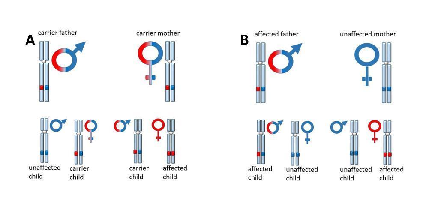
\includegraphics[scale=1]{inh_autosomal.eps}}
  \caption{\csentence{}Autosomal inheritance pattern with red disease allele.
(A) Recessive inheritance, both parents as heterozygous carriers with an unaffected:carrier:affected ratio of 1:2:1.
(B) Dominant inheritance, one parent affected with an unaffected:affected ratio of 1:1.\label{fig:inheritance}}
\vspace{1em}
  \centerline{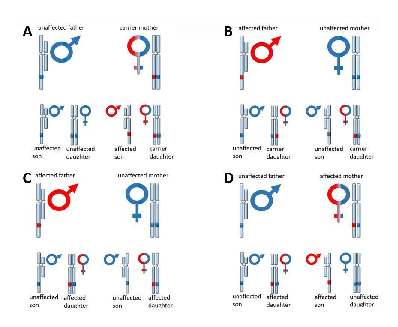
\includegraphics[scale=1]{inh_xlinked.eps}}
  \caption{\csentence{}X-linked inheritance pattern with a red disease allele. (A) Recessive inheritance, mother is a disease-carrier. A mother will pass her disease-allele to half of her offspring, resulting just sons to be affected. (B) Recessive inheritance, father is affected. A father will pass his disease-allele to all of his daughters resulting all of them to be a disease-carriers. (C) Dominant inheritance, father is affected. A father will pass his disease-allele to all his daughters resulting all of them to be affected. (D) Dominant inheritance, mother is affected. A mother will pass her disease-allele equally to daughters and sons, resulting half of them to be affected.\label{fig:inheritancex}}
\end{figure}

\begin{figure}[h!]
  \centerline{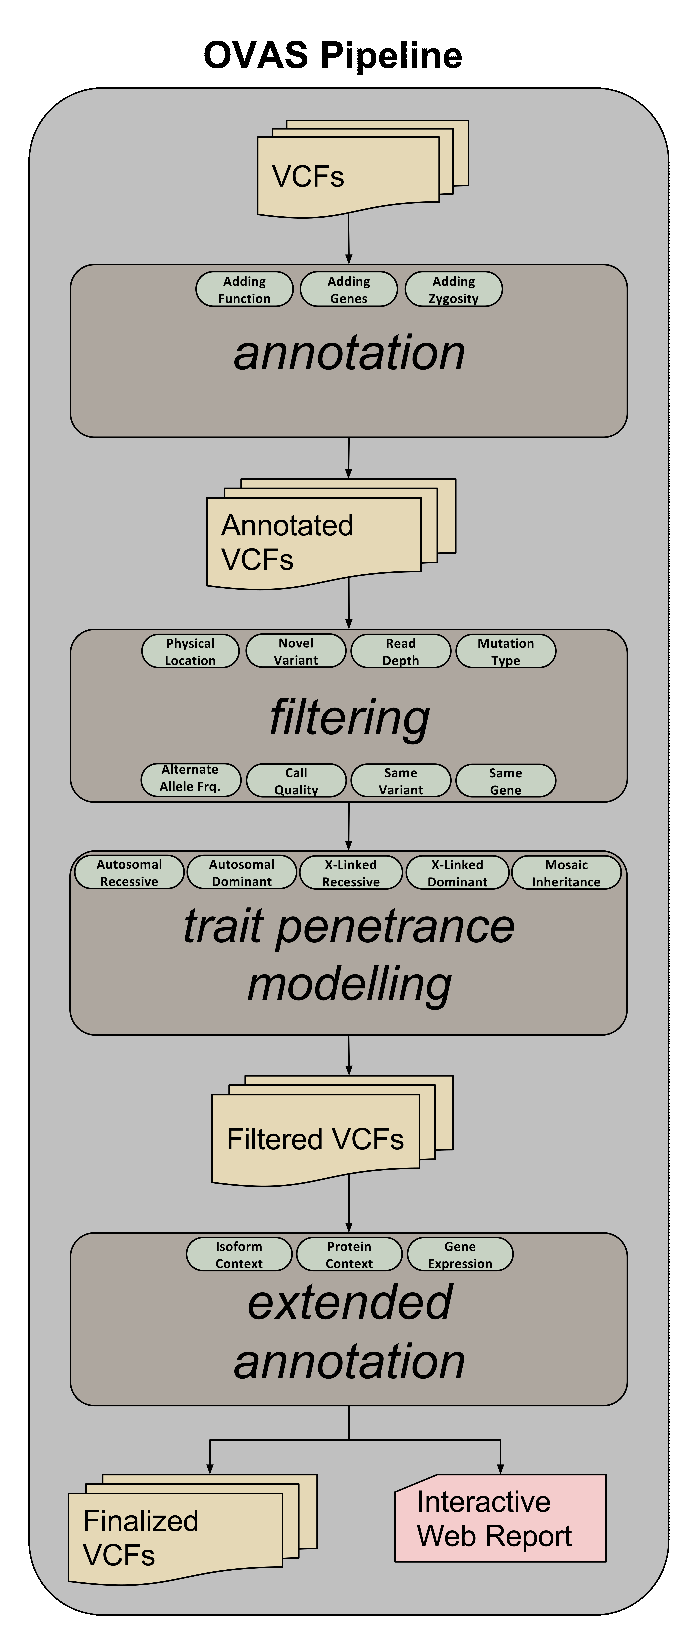
\includegraphics[scale=0.5]{pipeline_overall.eps}}
  \caption{\csentence{}Overall structure of the \app{} pipeline: VCF files as referenced by a pedigree file are fed into the pipeline in conjunction with static map and reference data; to be processed in turn by the core annotation, optional filtering, and additional annotation modules.\label{fig:structure}}
\end{figure}

\begin{figure}[h!]
  \centerline{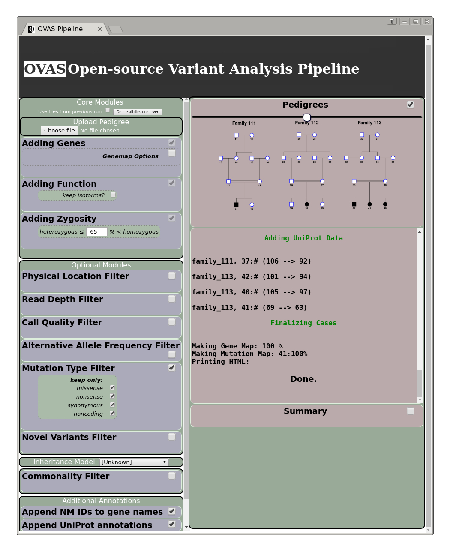
\includegraphics[scale=1]{pipe_3_final.eps}}
\caption{\csentence{}Web-interface displaying an ongoing analysis. The left sidebar shows the user-set configurations, and the central-right box displays the pedigrees used in the analysis stacked above a real-time progress box. Once complete, a summary will automatically open in a new browser tab.\label{fig:webend}}
\end{figure}
\begin{figure}[h!]
  \centerline{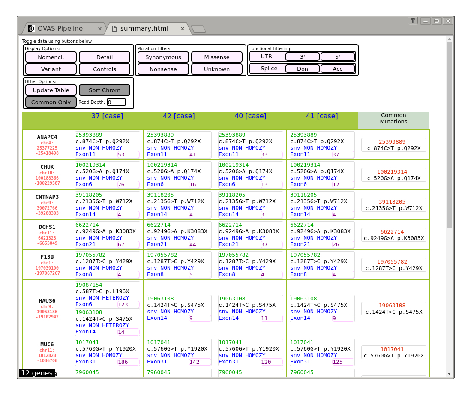
\includegraphics[scale=1]{report_small.eps}}
\caption{\csentence{}The summary tab which contains a comprehensive report of potential causative variants discovered in the analysis. The report is interactive and can perform dynamic filtering of discovered variants by toggling variants identified as synonymous, missense, nonsense, UTR (optionally 3' or 5'), and splice (optionally Donor or Acceptor).\label{fig:report}}
\end{figure}

\begin{figure}[h!]
  \centerline{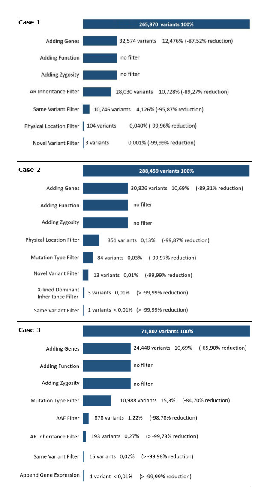
\includegraphics[scale=1]{control_result_total.eps}}
\caption{\csentence{}The progression of output variants through core annotation and filtering stages for each of the three separate cases.\label{fig:result}}
\end{figure}


%%%%%%%%%%%%%%%%%%%%%%%%%%%%%%%%%%%
%%                               %%
%% Tables                        %%
%%                               %%
%%%%%%%%%%%%%%%%%%%%%%%%%%%%%%%%%%%

%% Use of \listoftables is discouraged.
%%
\section*{Tables}

%% Results table
\begin{table}[h!]
\begin{tabular}{| c | *2c |} \hline %\toprule
%\emph{Pipeline} & \emph{Module} & \emph{Runtime} \\
%\emph{Stage} & \emph{Name} & \emph{(seconds)} \\
\emph{Pipeline Stage} & \emph{Module Name} & \emph{Runtime (seconds)} \\
\hline
% A multirow would be more benefial here
% but let's keep package req down for now
             & Adding Genes     & 125\\
Annotation   & Adding Function & 28.7\\
             & Adding Zygosity & 0.81\\
\hline
             & Physical Location Filter & 1.02 \\
             & Read Depth Filter        & 1.26 \\
             & Call Quality Filter      & 0.93\\
Filtering    & AAF Filter               & 432\\
             & Mutation Type Filter     & 1.08\\
             & Novel Variant Filter     & 1.12\\
             & Same Gene Filter       & 22.5\\
             & Same Variant Filter    & 26.1\\
\hline
             & AD Inheritance    & 0.83\\
 Trait       & AR Inheritance    & 1.22\\
Penetrance   & XD Inheritance    & 0.74\\
  Model      & XR Inheritance    & 1.39\\
             & Mosaicism         & 0.94\\
\hline
                 & Isoform Context      & 2.28\\
   Extended      & Protein Context      & 4.10\\
 Annotation      & Gene Expression      & 145\\
\hline
%\botrule
\end{tabular}
\vspace{1ex}
\caption{Average single-core runtimes of VCF files containing 50,000 variants passing individually through all filters with timings for each Annotation, Filtering, and Extended Annotation modules. Trait Penetrance module timings are based on three VCFs consisting of a parent-offspring trio. Tests were run on a 2GHz dual-core processor with 4GB RAM.}\label{table:results}
\end{table}




%%%%%%%%%%%%%%%%%%%%%%%%%%%%%%%%%%%
%%                               %%
%% Additional Files              %%
%%                               %%
%%%%%%%%%%%%%%%%%%%%%%%%%%%%%%%%%%%

\end{backmatter}
\end{document}
